\documentclass[11pt,a4paper]{article}
\usepackage[T1]{fontenc}
\usepackage[portuguese]{babel}
\usepackage[utf8]{inputenc}
\inputencoding{utf8}
\usepackage{url}
%\usepackage{siunitx} % Provides the \SI{}{} and \si{} command for typesetting SI units
\usepackage{graphicx} % Required for the inclusion of images
\usepackage{caption}
\usepackage{subcaption}
\usepackage{natbib} % Required to change bibliography style to APA
\usepackage{enumerate}
\usepackage{amsmath} % Required for some math elements 
\usepackage{graphicx}
\usepackage{epstopdf} %use postscript
\usepackage{float}
\usepackage{a4wide}
\usepackage{amsmath}
\usepackage{amsfonts}
\usepackage{wrapfig}
\usepackage{tikz}
\usepackage{multicol}
\usetikzlibrary{shapes,arrows,positioning,calc}
\usepackage{amsthm} % Math packages
%\usepackage[headheight=14pt]{geometry}
\usepackage{sectsty} % Allows customizing section commands
\usepackage{fancyhdr} % Custom headers and footers
%\usepackage[margin=1in]{geometry} % Change margin
\usepackage{longtable}

\pagestyle{fancyplain} % Makes all pages in the document conform to the custom headers and footers
%\fancyhead{} % No page header - if you want one, create it in the same way as the footers below
\fancyhead[L]{Relatório Preliminar}% Empty left footer
\fancyhead[R]{Inteligência Computacional} % Empty center footer
\fancyfoot[C]{\thepage} 								% Page numbering for right footer
\numberwithin{equation}{section}


\begin{document}


\begin{titlepage}

\vspace*{\fill}
 
\newcommand{\HRule}{\rule{\linewidth}{0.5mm}} 	% Defines a new command for the horizontal lines, change thickness here

\center 												% Center everything on the page
 
%----------------------------------------------------------------------------------------
%   LOGO SECTION
%----------------------------------------------------------------------------------------


\includegraphics[scale=0.3]{./minerva}\\[1cm] % Include a department/university logo - this will require the graphicx package
 
%----------------------------------------------------------------------------------------
%   HEADING SECTIONS
%----------------------------------------------------------------------------------------

\textsc{\LARGE Universidade Federal do Rio de Janeiro}\\[1.5cm] % Name of your university/college
\textsc{\Large Inteligência Computacional}\\[0.5cm] % Major heading such as course name
%\textsc{\large   }\\[0.5cm] % Minor heading such as course title

%----------------------------------------------------------------------------------------
%   TITLE SECTION
%----------------------------------------------------------------------------------------

\HRule 
\\[0.8cm]
{ \huge \bfseries  Breast Cancer Wisconsin  }\\[0.4cm] % Title of your document
\HRule \\[1.5cm]
 
%----------------------------------------------------------------------------------------
%   AUTHOR SECTION
%----------------------------------------------------------------------------------------

\begin{minipage}{0.4\textwidth}
\begin{flushleft} \large
\emph{Nomes:}\\
Aramys Almeida Matos \\
Luís Gustavo Oliveira Silva 
\end{flushleft}
\end{minipage}
~
\begin{minipage}{0.4\textwidth}
\begin{flushright} \large
\emph{Professor:} \\
Alexandre Evsukoff  % Supervisor's Name
\end{flushright}
\end{minipage}\\[4cm]
%----------------------------------------------------------------------------------------
%   DATE SECTION
%----------------------------------------------------------------------------------------


%----------------------------------------------------------------------------------------

%\vfill % Fill the rest of the page with whitespace
\vspace*{\fill}
\end{titlepage}
\section{Introdução}
Este trabalho será desenvolvido sobre o \textit{dataset Breast Cancer Wisconsin (Diagnostic)}. Este \textit{dataset} possui como variáveis características computadas a partir de imagens digitalizadas de exames de mama por punção aspirativa por agulha fina. Os dados descrevem características do núcleo das células presentes na imagem. 
\section{Caracterização}

\subsection{Dados}
%O dataset possui os seguintes dados.

%\begin{itemize}
%\item ID do paciente.
%\item 
%\end{itemize}

Inicialmente é importante ressaltar que o conjunto de dados gerado pelos exames é tridimensional. Para cada registro (paciente) existe um conjunto de células, cada uma com os seguintes atributos.

\begin{enumerate}
\item Raio (média das distâncias do centro para pontos no perímetro)
\item Textura
\item Perímetro
\item Área
\item Suavidade
\item Compacidade
\item Concavidade
\item Pontos côncavos
\item Simetria
\item Dimensão Fractal
\end{enumerate}

De forma a eliminar a terceira dimensão (do conjunto de células), para cada conjunto de células o \textit{UCI Machine Learning} forneceu o dataset com valores de média, desvio(erro) padrão e o pior valor dos atributos no universo das células, resultando em 30 variáveis de entrada. O dataset conforme obtido possui as variáveis como segue:

\begin{multicols}{3}
\begin{itemize}
    \item radius\_mean	
    \item texture\_mean
    \item perimeter\_mean
    \item area\_mean
    \item smoothness\_mean
    \item compactness\_mean
    \item concavity\_mean
    \item concave points\_mean
    \item symmetry\_mean
    \item fractal\_dimension\_mean
    \item radius\_se
    \item texture\_se
    \item perimeter\_se
    \item area\_se
    \item smoothness\_se
    \item compactness\_se
    \item concavity\_se
    \item concave points\_se
    \item symmetry\_se
    \item fractal\_dimension\_se
    \item radius\_worst
    \item texture\_worst
    \item perimeter\_worst
    \item area\_worst
    \item smoothness\_worst
    \item compactness\_worst
    \item concavity\_worst
    \item concave points\_worst
    \item symmetry\_worst
    \item fractal\_dimension\_worst
\end{itemize}
\end{multicols}

A variável de saída é o diagnóstico (maligno ou benigno codificados como $-1$ e $1$ respectivamente). Existe uma coluna com o ID do paciente que será eliminada ser irrelevante. O dataset apresenta 357 amostras benignas e 212 amostras malignas. 

%\newpage
\subsection{Estatísticas Básicas e Histogramas}

\begin{itemize}
\item Radius
\begin{figure}[H]
\centering
  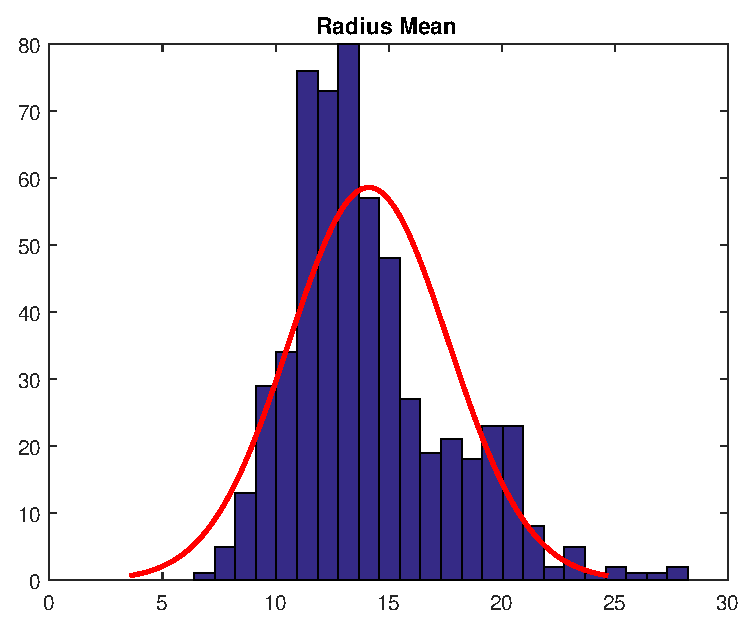
\includegraphics[width=.4\linewidth]{./img/radius_mean}
  \captionof{figure}{Mean}
  \label{fig:test1}
\end{figure}%

\begin{figure}[H]
\centering
\begin{minipage}{.4\textwidth}
  \centering
  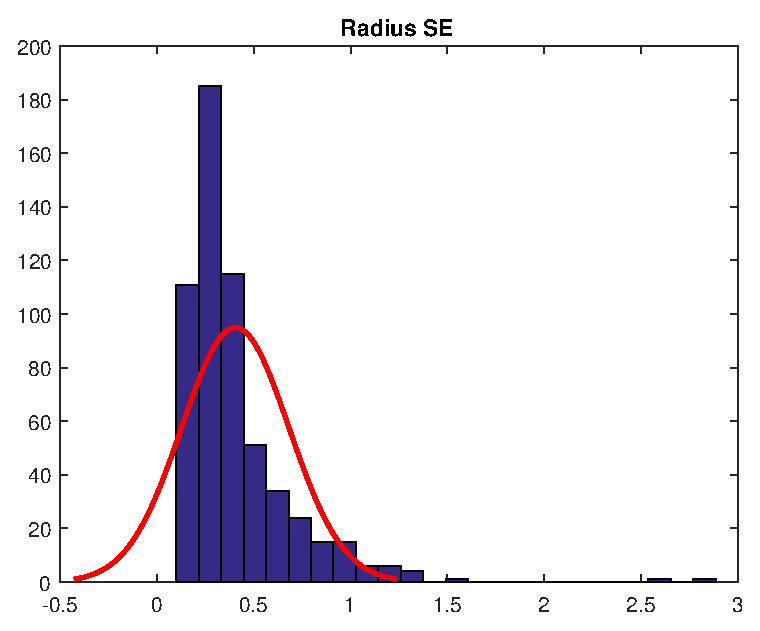
\includegraphics[width=\linewidth]{./img/radius_se}
  \captionof{figure}{Standard Error}
  \label{fig:test1}
\end{minipage}%
\begin{minipage}{.4\textwidth}
  \centering
  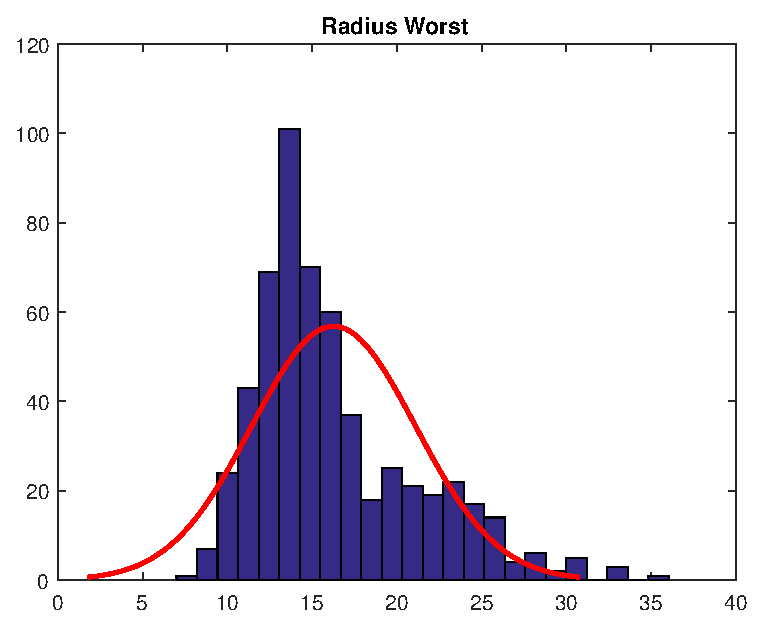
\includegraphics[width=\linewidth]{./img/radius_worst}
  \captionof{figure}{Worst}
  \label{fig:test2}
\end{minipage}
\end{figure}

\begin{table}[H]
\centering
\caption{Radius}
\label{my-label}
\begin{tabular}{lllll}
\hline
              & radius\_mean & radius\_se & radius\_worst &  \\
\hline
Máximo        & 28.11        & 2.873      & 36.04         &  \\
Mínimo        & 6.981        & 0.1115     & 7.93          &  \\
Média         & 14.12729     & 0.405172   & 16.26919      &  \\
Desvio padrão & 3.524049     & 0.277313   & 4.833242      &  \\
Percentil 25  & 11.7         & 0.2324     & 13.01         &  \\
Percentil 50  & 13.37        & 0.3242     & 14.97         &  \\
Percentil 75  & 15.78        & 0.4789     & 18.79         &  \\
\hline
\end{tabular}
\end{table}


Análise: Para a variável Radius mean, vemos que a maioria de seus valores se concentram mais proximos da média que é 14,13.
Para Radius Standard Error, também têm um coportamento semelhante a uma função de cauda longa, porém não temos a presença de valores no intervalo entre 1,6 e 2,4.
Já para a variável Radius Worst, tem um comportamento semelhante à variável Radius mean.

\item Texture
\begin{figure}[H]
\centering
  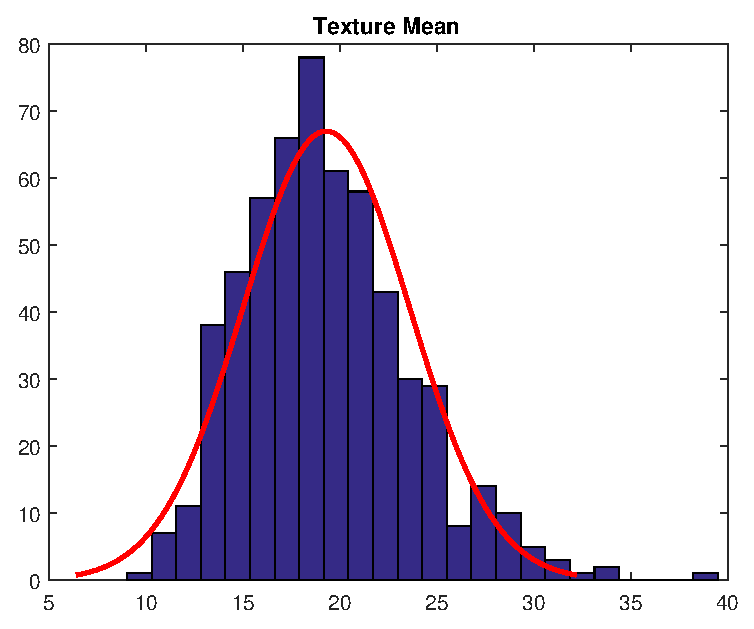
\includegraphics[width=.4\linewidth]{./img/texture_mean}
  \captionof{figure}{Mean}
  \label{fig:test1}
\end{figure}%

\begin{figure}[H]
\centering
\begin{minipage}{.4\textwidth}
  \centering
  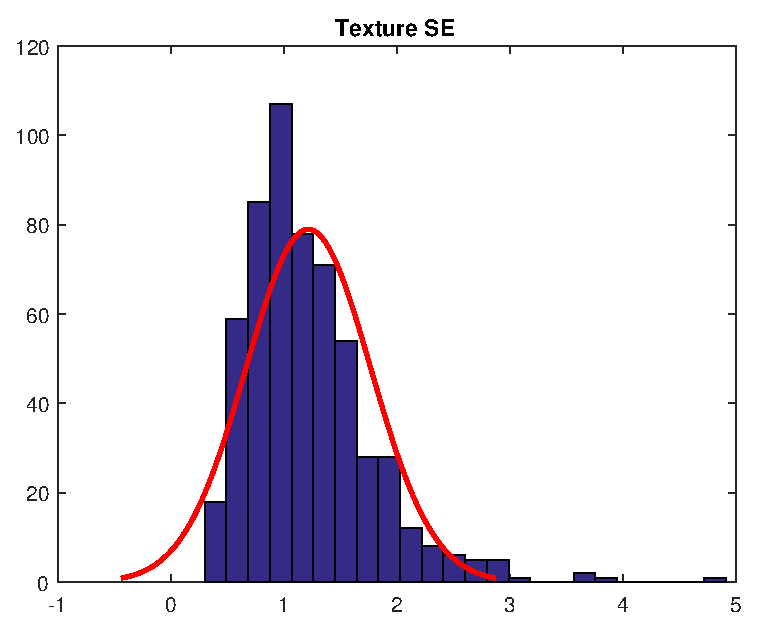
\includegraphics[width=\linewidth]{./img/texture_se}
  \captionof{figure}{Standard Error}
  \label{fig:test1}
\end{minipage}%
\begin{minipage}{.4\textwidth}
  \centering
  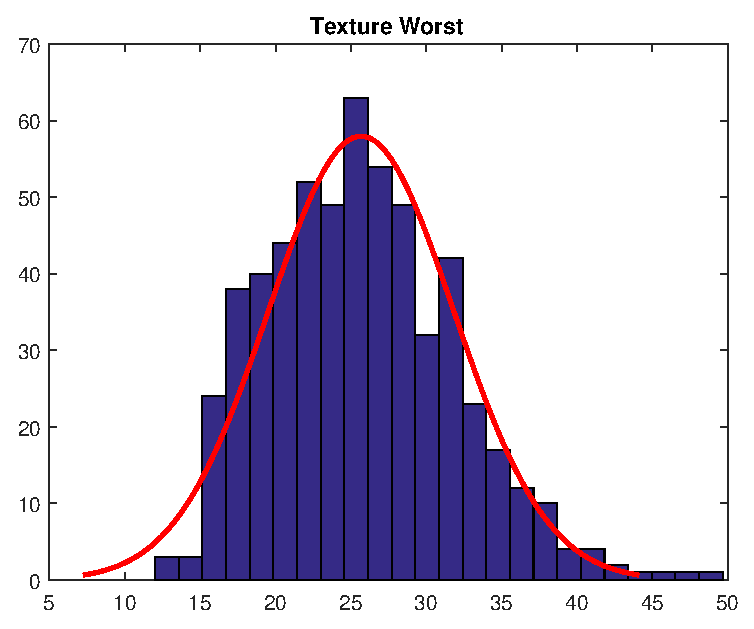
\includegraphics[width=\linewidth]{./img/texture_worst}
  \captionof{figure}{Worst}
  \label{fig:test2}
\end{minipage}
\end{figure}

\begin{table}[H]
\centering
\caption{Texture}
\label{my-label}
\begin{tabular}{lllll}
\hline
              & texture\_mean & texture\_se & texture\_worst &  \\ \hline
Máximo        & 39.28         & 4.885       & 49.54          &  \\
Mínimo        & 9.71          & 0.3602      & 12.02          &  \\
Média         & 19.28964851   & 1.216853427 & 25.67722       &  \\
Desvio padrão & 4.301035768   & 0.551648393 & 6.146258       &  \\
Percentil 25  & 16.17         & 0.8339      & 21.08          &  \\
Percentil 50  & 18.84         & 1.108       & 25.41          &  \\
Percentil 75  & 21.8          & 1.474       & 29.72          & \\ \hline
\end{tabular}
\end{table}

Análise: Podemos perceber que a variável Texture Mean, tem um comportamento que lembra a uma função Gaussiana, que de certa forma é espelhada em realação a média, com a exceção dos outliers. Em Texture Standart Error, a média é 1,22  e seus valores estão localizados proóximos á média, porém temos uma certa quantidade de valores distantes, mesmo considerando o desvio parão, e um valor máximo muito alto. Em Texture Worst, vemos que seu comportamento se assemelha a Texture Mean.


\item Perimeter
\begin{figure}[H]
\centering
  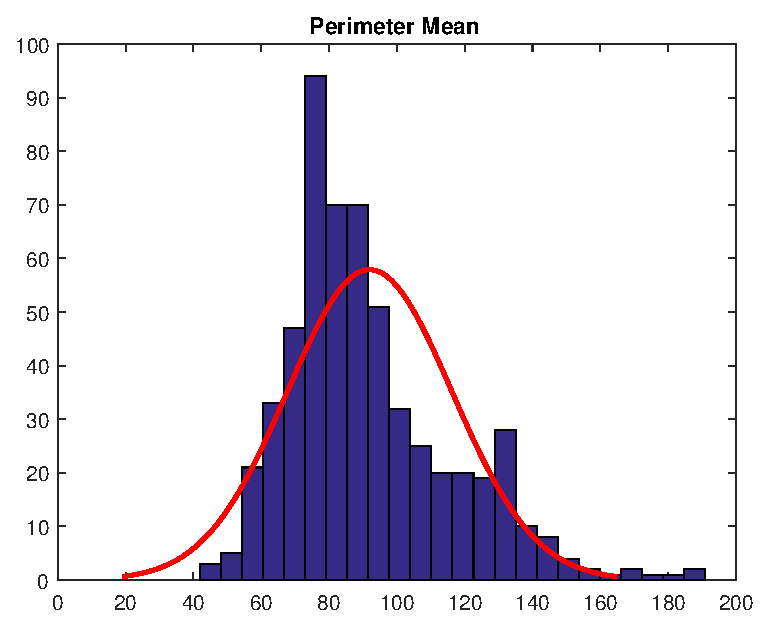
\includegraphics[width=.4\linewidth]{./img/perimeter_mean}
  \captionof{figure}{Mean}
  \label{fig:test1}
\end{figure}%

\begin{figure}[H]
\centering
\begin{minipage}{.4\textwidth}
  \centering
  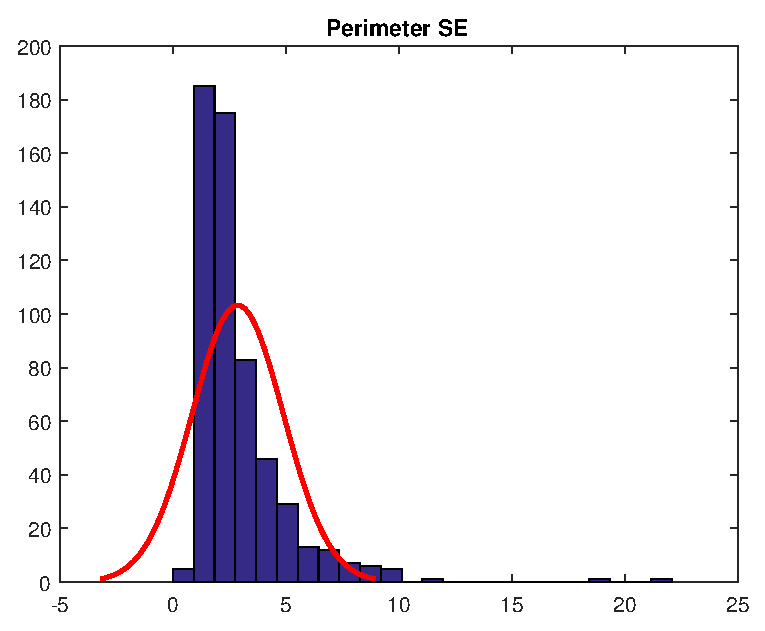
\includegraphics[width=\linewidth]{./img/perimeter_se}
  \captionof{figure}{Standard Error}
  \label{fig:test1}
\end{minipage}%
\begin{minipage}{.4\textwidth}
  \centering
  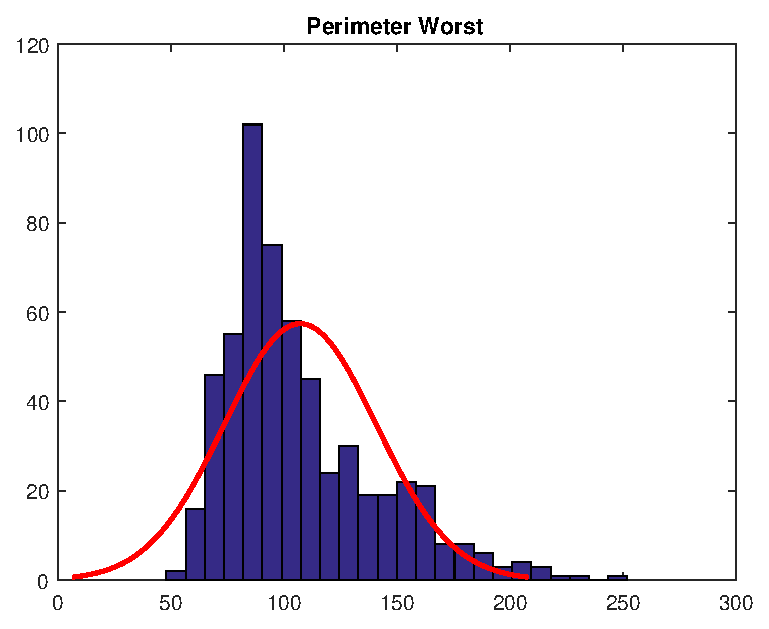
\includegraphics[width=\linewidth]{./img/perimeter_worst}
  \captionof{figure}{Worst}
  \label{fig:test2}
\end{minipage}
\end{figure}


\begin{table}[H]
\centering
\caption{Perimeter}
\label{my-label}
\begin{tabular}{lllll} \hline
              & perimeter\_mean & perimeter\_se & perimeter\_worst &  \\ \hline
Máximo        & 188.5           & 21.98         & 251.2            &  \\
Mínimo        & 43.79           & 0.757         & 50.41            &  \\
Média         & 91.96903339     & 2.866059227   & 107.2612         &  \\
Desvio padrão & 24.29898104     & 2.021854554   & 33.60254         &  \\
Percentil 25  & 75.17           & 1.606         & 84.11            &  \\
Percentil 50  & 86.24           & 2.287         & 97.66            &  \\
Percentil 75  & 104.1           & 3.357         & 125.4            & \\ \hline
\end{tabular}
\end{table}

Análise: Em Perimeter Standard Error, vemos a presença de outliers, como por exemplo o valor máximo que é 21,98,  enquanto sua média é 2.87. E em Perimeter Worst, vemos que possui um desvio padrão alto e seus valores estão distribuídos de forma distante da média.


\item Area
\begin{figure}[H]
\centering
  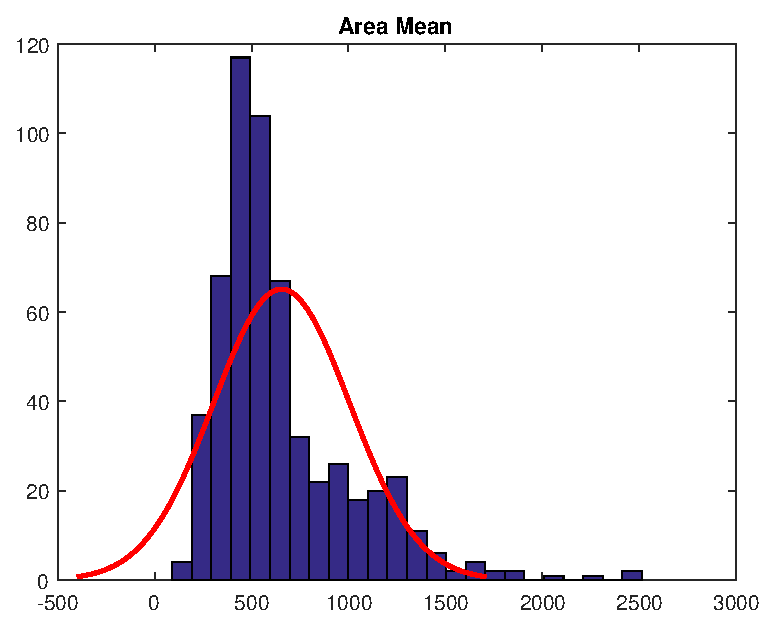
\includegraphics[width=.4\linewidth]{./img/area_mean}
  \captionof{figure}{Mean}
  \label{fig:test1}
\end{figure}%

\begin{figure}[H]
\centering
\begin{minipage}{.4\textwidth}
  \centering
  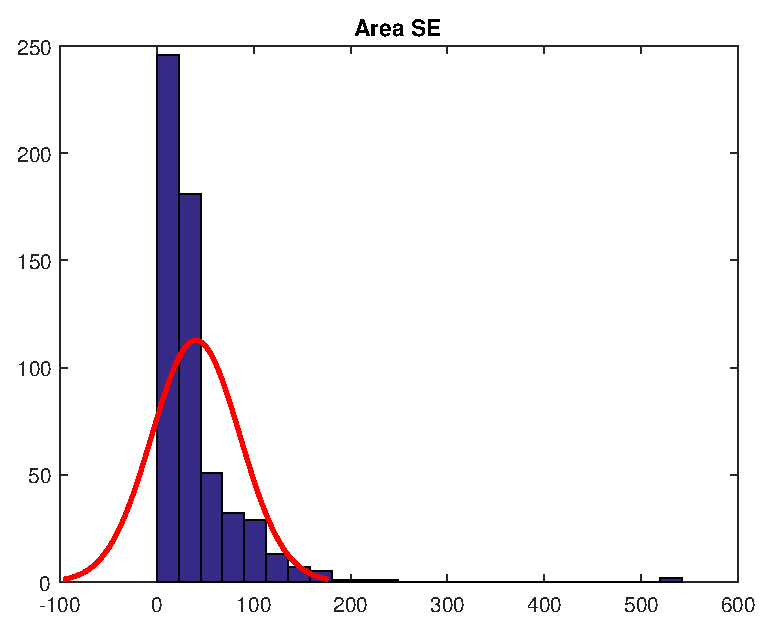
\includegraphics[width=\linewidth]{./img/area_se}
  \captionof{figure}{Standard Error}
  \label{fig:test1}
\end{minipage}%
\begin{minipage}{.4\textwidth}
  \centering
  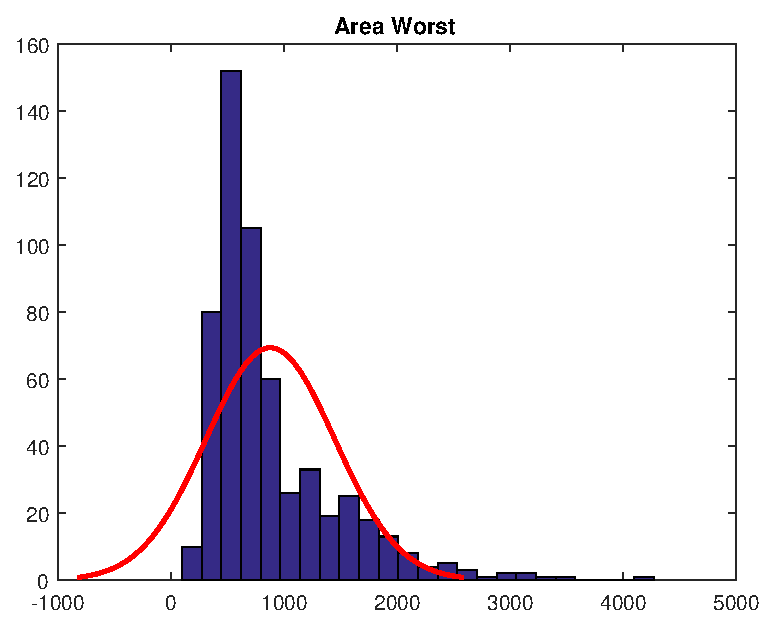
\includegraphics[width=\linewidth]{./img/area_worst}
  \captionof{figure}{Worst}
  \label{fig:test2}
\end{minipage}
\end{figure}

\begin{table}[H]
\centering
\caption{Area}
\label{my-label}
\begin{tabular}{lllll} \hline
              & area\_mean  & area\_se    & area\_worst &  \\ \hline
Máximo        & 2501        & 542.2       & 4254        &  \\
Mínimo        & 143.5       & 6.802       & 185.2       &  \\
Média         & 654.8891037 & 40.33707909 & 880.5831283 &  \\
Desvio padrão & 351.9141292 & 45.49100552 & 569.3569927 &  \\
Percentil 25  & 420.3       & 17.85       & 515.3       &  \\
Percentil 50  & 551.1       & 24.53       & 686.5       &  \\
Percentil 75  & 782.7       & 45.19       & 1084        &  \\ \hline
\end{tabular}
\end{table}

Análise: Na variável Area Mean, vemos que ela possui um desvio padrão grande, sendo maior que a metade da média, assim como em Area Worst. Em Area Standard Error, vemos que a variável tem um compartamento semelhante a uma função de cauda longa e temos uma valor bem distante que é o valor máximo ( 2501,00). 


\item Smoothness
\begin{figure}[H]
\centering
  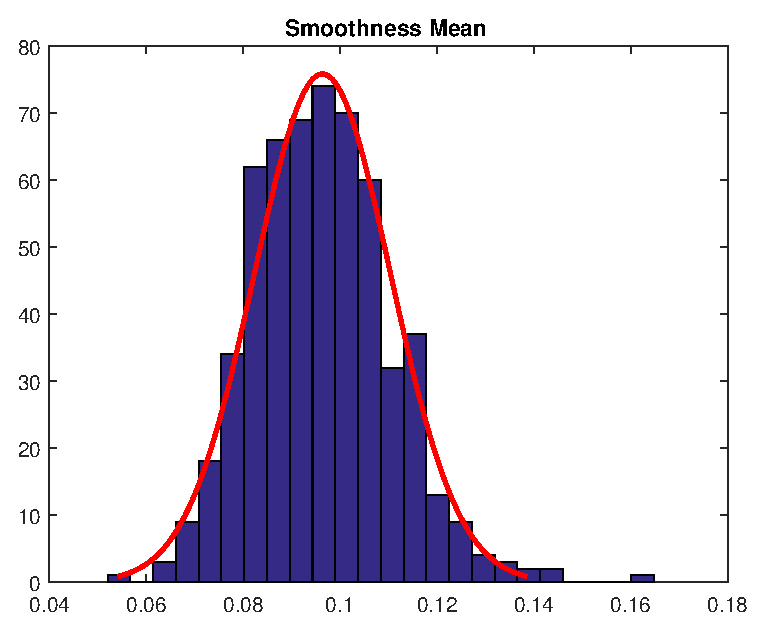
\includegraphics[width=.4\linewidth]{./img/smoothness_mean}
  \captionof{figure}{Mean}
  \label{fig:test1}
\end{figure}%

\begin{figure}[H]
\centering
\begin{minipage}{.4\textwidth}
  \centering
  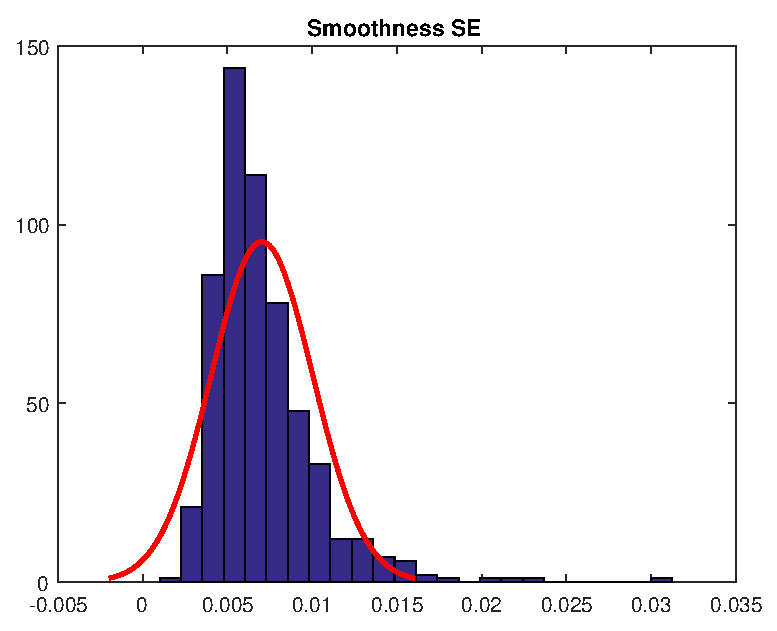
\includegraphics[width=\linewidth]{./img/smoothness_se}
  \captionof{figure}{Standard Error}
  \label{fig:test1}
\end{minipage}%
\begin{minipage}{.4\textwidth}
  \centering
  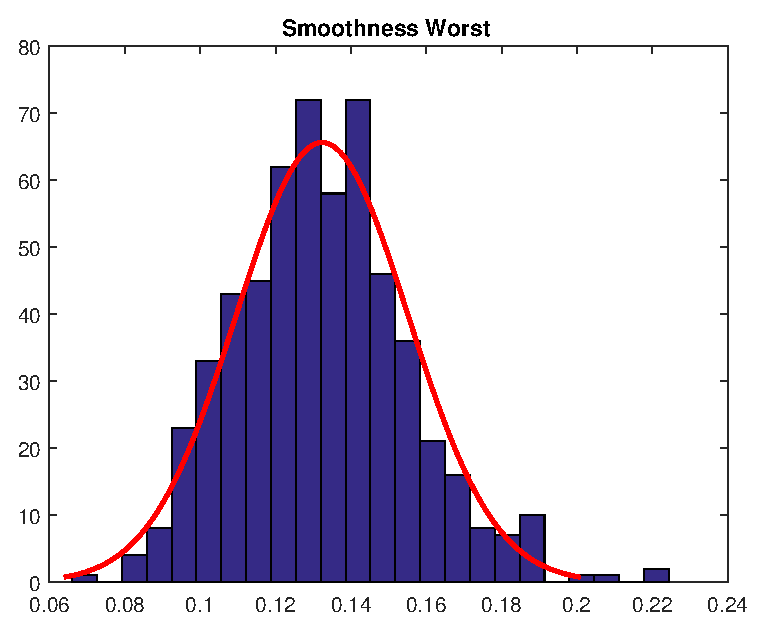
\includegraphics[width=\linewidth]{./img/smoothness_worst}
  \captionof{figure}{Worst}
  \label{fig:test2}
\end{minipage}
\end{figure}

\begin{table}[H]
\centering
\caption{Smoothness}
\label{my-label}
\begin{tabular}{lllll} \hline
              & smoothness\_mean & smoothness\_se & smoothness\_worst &  \\ \hline
Máximo        & 0.1634           & 0.03113        & 0.2226            &  \\
Mínimo        & 0.05263          & 0.001713       & 0.07117           &  \\
Média         & 0.096360281      & 0.007040979    & 0.132368594       &  \\
Desvio padrão & 0.014064128      & 0.003002518    & 0.022832429       &  \\
Percentil 25  & 0.08637          & 0.005169       & 0.1166            &  \\
Percentil 50  & 0.09587          & 0.00638        & 0.1313            &  \\
Percentil 75  & 0.1053           & 0.008146       & 0.146             & \\ \hline
\end{tabular}
\end{table}

Análise: Podemos ver que tanto Smoothness Mean quanto em Worst, elas tem uma aparência semelhante a uma função Gaussiana e possuem um desvio padrão pequeno, já em Smoothness Standard Error, vemos que ela possui um desvio padrão alto e existe a presença de outliers como o seu valor máximo (0,16340).


\item Compactness
\begin{figure}[H]
\centering
  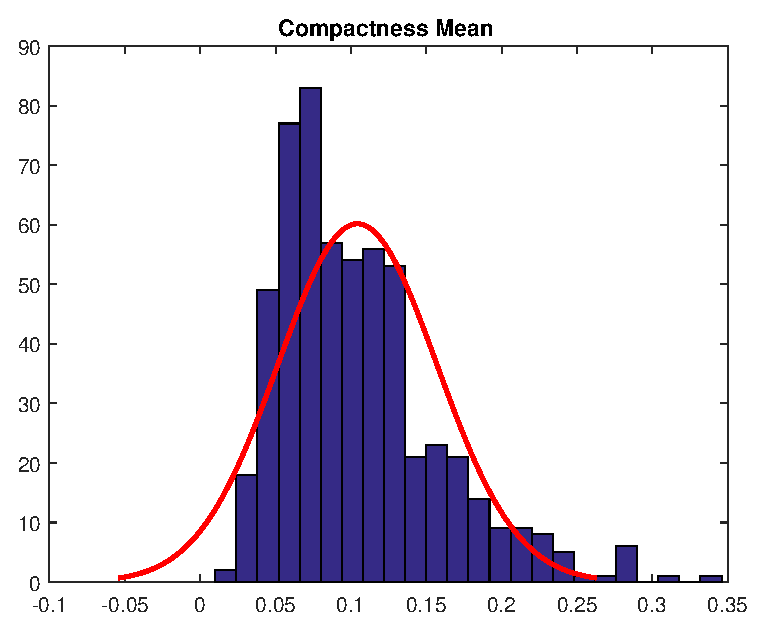
\includegraphics[width=.4\linewidth]{./img/compactness_mean}
  \captionof{figure}{Mean}
  \label{fig:test1}
\end{figure}%


\begin{figure}[H]
\centering
\begin{minipage}{.4\textwidth}
  \centering
  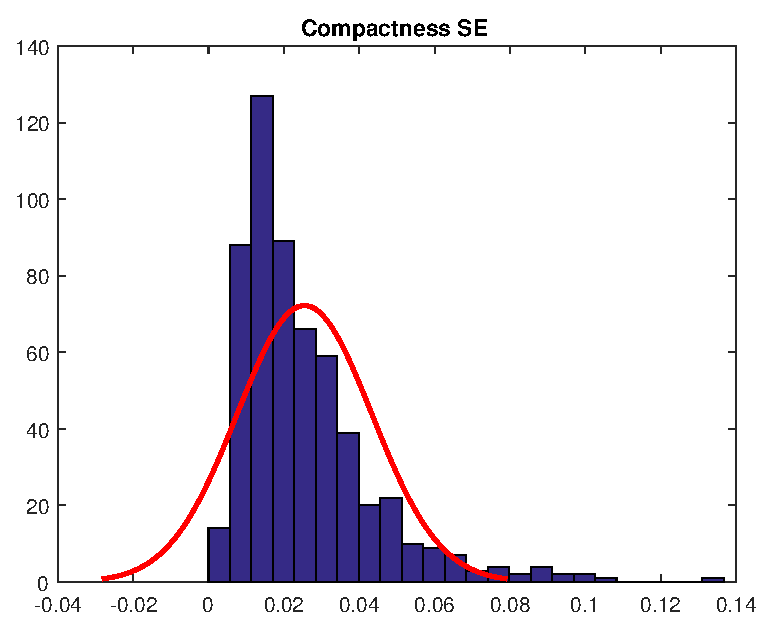
\includegraphics[width=\linewidth]{./img/compactness_se}
  \captionof{figure}{Standard Error}
  \label{fig:test1}
\end{minipage}%
\begin{minipage}{.4\textwidth}
  \centering
  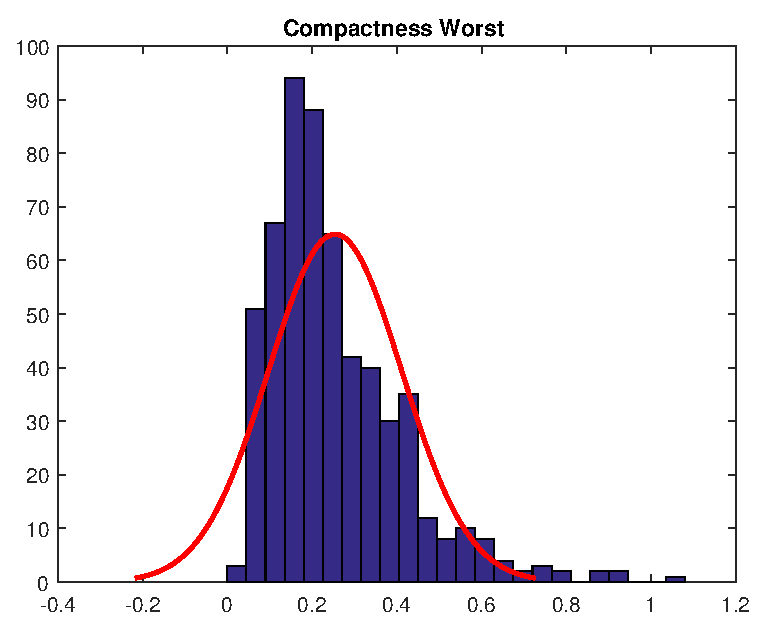
\includegraphics[width=\linewidth]{./img/compactness_worst}
  \captionof{figure}{Worst}
  \label{fig:test2}
\end{minipage}
\end{figure}

\begin{table}[H]
\centering
\caption{Compactness}
\label{my-label}
\begin{tabular}{lllll}\hline
              & compactness\_mean & compactness\_se & compactness\_worst &  \\ \hline
Máximo        & 0.3454            & 0.1354          & 1.058              &  \\
Mínimo        & 0.01938           & 0.002252        & 0.02729            &  \\
Média         & 0.104340984       & 0.025478139     & 0.254265           &  \\
Desvio padrão & 0.052812758       & 0.017908179     & 0.157336           &  \\
Percentil 25  & 0.06492           & 0.01308         & 0.1472             &  \\
Percentil 50  & 0.09263           & 0.02045         & 0.2119             &  \\
Percentil 75  & 0.1304            & 0.03245         & 0.3391             &  \\ \hline
\end{tabular}
\end{table}

Análise: Aqui percebemos que as 3 variáveis possuem um desvio padrão alto e seus valores máximos se destoam bantante.

\item Concavity
\begin{figure}[H]
\centering
  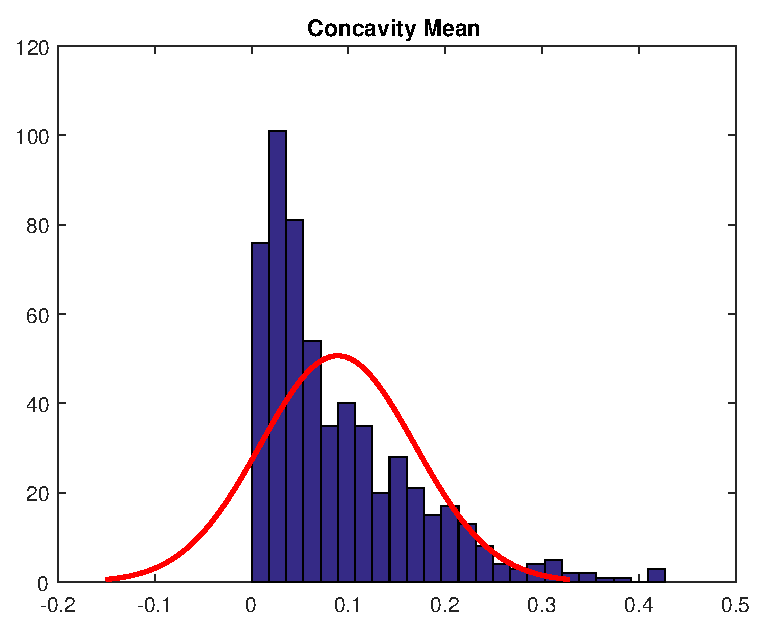
\includegraphics[width=.4\linewidth]{./img/concavity_mean}
  \captionof{figure}{Mean}
  \label{fig:test1}
\end{figure}%


\begin{figure}[H]
\centering
\begin{minipage}{.4\textwidth}
  \centering
  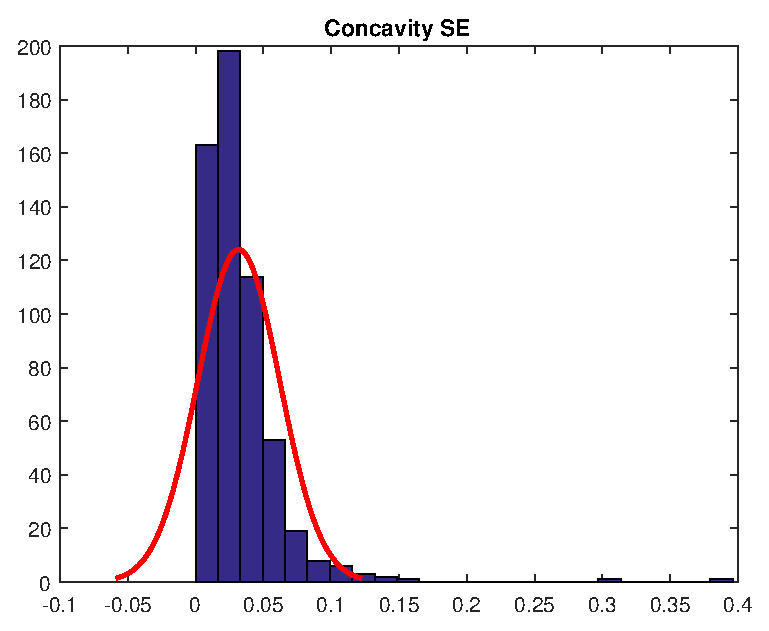
\includegraphics[width=\linewidth]{./img/concavity_se}
  \captionof{figure}{Standard Error}
  \label{fig:test1}
\end{minipage}%
\begin{minipage}{.4\textwidth}
  \centering
  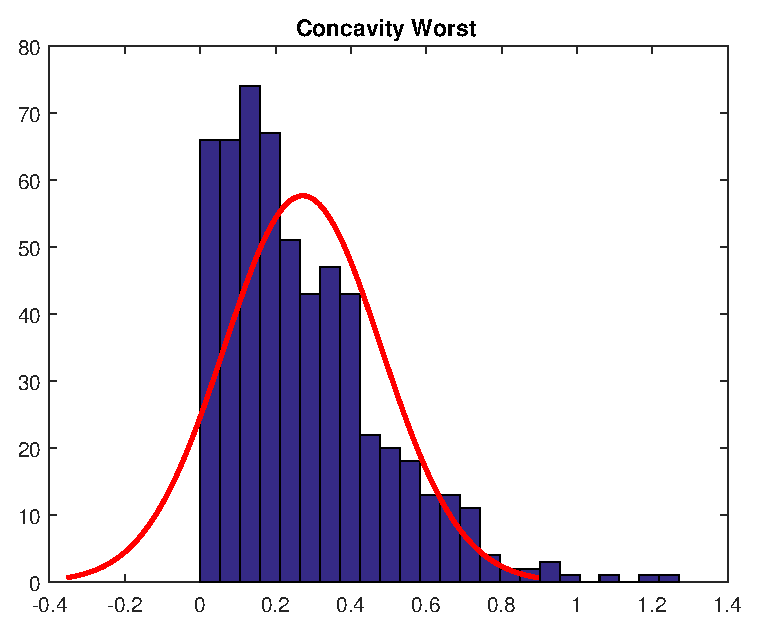
\includegraphics[width=\linewidth]{./img/concavity_worst}
  \captionof{figure}{Worst}
  \label{fig:test2}
\end{minipage}
\end{figure}

\begin{table}[H]
\centering
\caption{Concavity}
\label{my-label}
\begin{tabular}{lllll} \hline
              & concavity\_mean & concavity\_se & concavity\_worst &  \\ \hline
Máximo        & 0.4268          & 0.396         & 1.252            &  \\
Mínimo        & 0               & 0             & 0                &  \\
Média         & 0.088799316     & 0.031893716   & 0.272188483      &  \\
Desvio padrão & 0.079719809     & 0.03018606    & 0.208624281      &  \\
Percentil 25  & 0.02956         & 0.01509       & 0.1145           &  \\
Percentil 50  & 0.06154         & 0.02589       & 0.2267           &  \\
Percentil 75  & 0.1307          & 0.04205       & 0.3829           & \\ \hline
\end{tabular}
\end{table}

Análise: Nas 3 variáveis percebemos que o seus valores se concentram mais proximos de 0 e a ocorrência desses valores vão decaindo conforme se afastam de 0.

\item Concave points
\begin{figure}[H]
\centering
  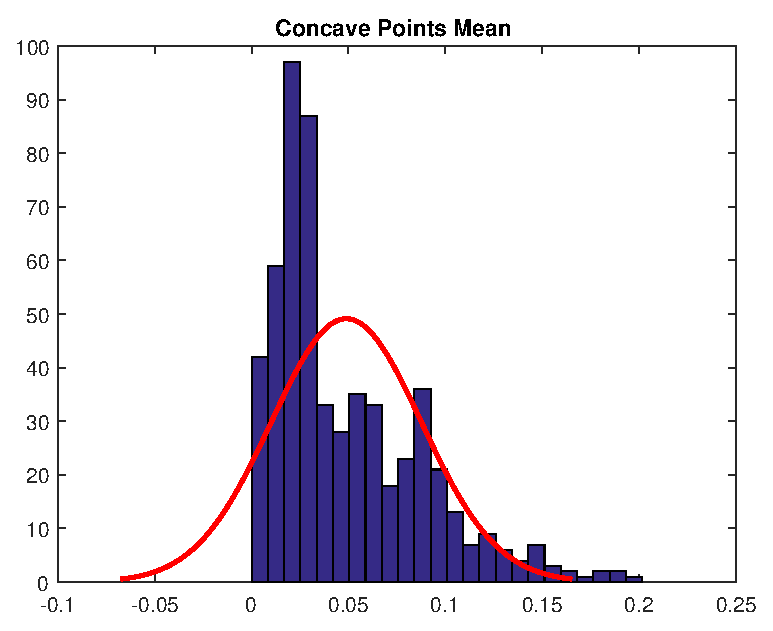
\includegraphics[width=.4\linewidth]{./img/concave_points_mean}
  \captionof{figure}{Mean}
  \label{fig:test1}
\end{figure}%

\begin{figure}[H]
\centering
\begin{minipage}{.4\textwidth}
  \centering
  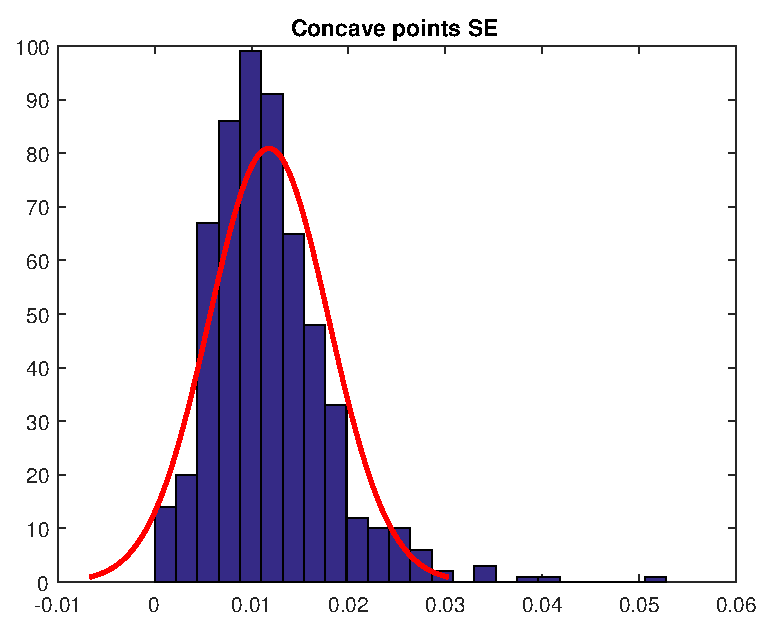
\includegraphics[width=\linewidth]{./img/concave_points_se}
  \captionof{figure}{Standard Error}
  \label{fig:test1}
\end{minipage}%
\begin{minipage}{.4\textwidth}
  \centering
  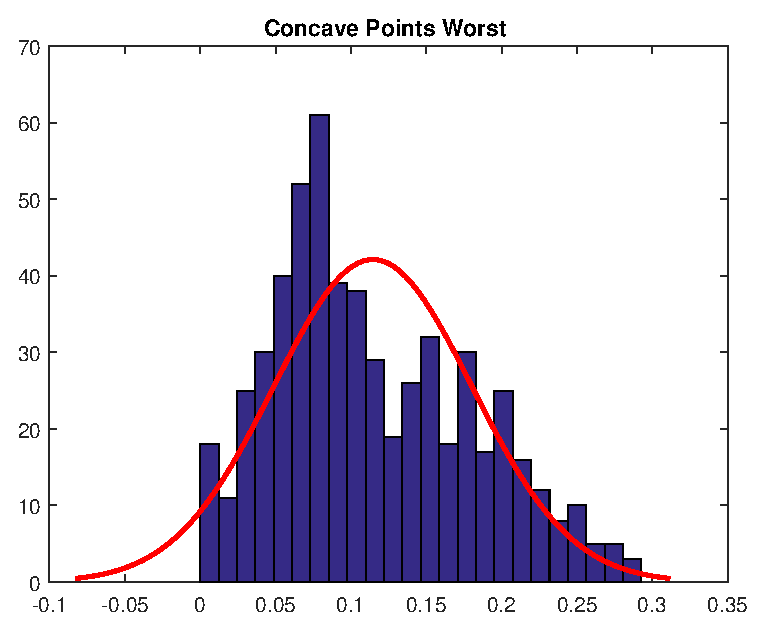
\includegraphics[width=\linewidth]{./img/concave_points_worst}
  \captionof{figure}{Worst}
  \label{fig:test2}
\end{minipage}
\end{figure}

\begin{table}[H]
\centering
\caption{Concave points}
\label{my-label}
\begin{tabular}{lllll} \hline
              & concave points\_mean & concave points\_se & concave points\_worst &  \\ \hline
Máximo        & 0.2012               & 0.05279            & 0.291                 &  \\
Mínimo        & 0                    & 0                  & 0                     &  \\
Média         & 0.048919146          & 0.011796           & 0.114606              &  \\
Desvio padrão & 0.038802845          & 0.00617            & 0.065732              &  \\
Percentil 25  & 0.02031              & 0.007638           & 0.06493               &  \\
Percentil 50  & 0.0335               & 0.01093            & 0.09993               &  \\
Percentil 75  & 0.074                & 0.01471            & 0.1614                &  \\ \hline
\end{tabular}
\end{table}

Análise: Aqui vemos que a variável Cancave points mean, tem um comportamento semelhante  à uma função de cauda longa e que a variável Cancave Points Standard Error possui alguns outliers,  como o valor máximo por exemplo.

\item Symmetry
\begin{figure}[H]
\centering
  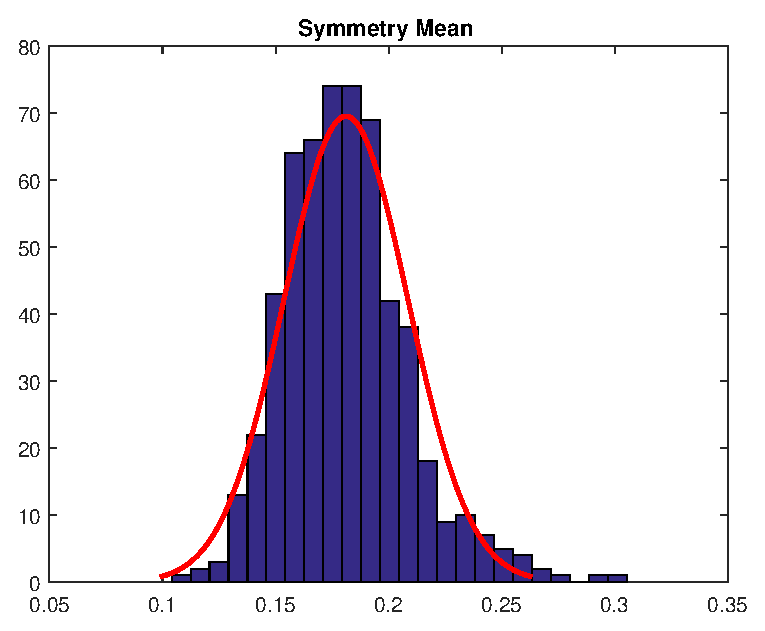
\includegraphics[width=.4\linewidth]{./img/symmetry_mean}
  \captionof{figure}{Mean}
  \label{fig:test1}
\end{figure}%

\begin{figure}[H]
\centering
\begin{minipage}{.4\textwidth}
  \centering
  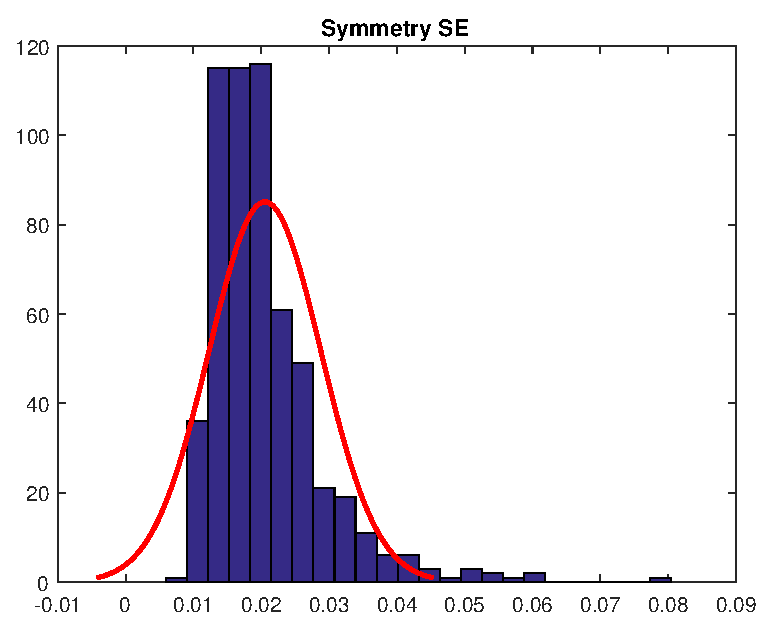
\includegraphics[width=\linewidth]{./img/symmetry_se}
  \captionof{figure}{Standard Error}
  \label{fig:test1}
\end{minipage}%
\begin{minipage}{.4\textwidth}
  \centering
  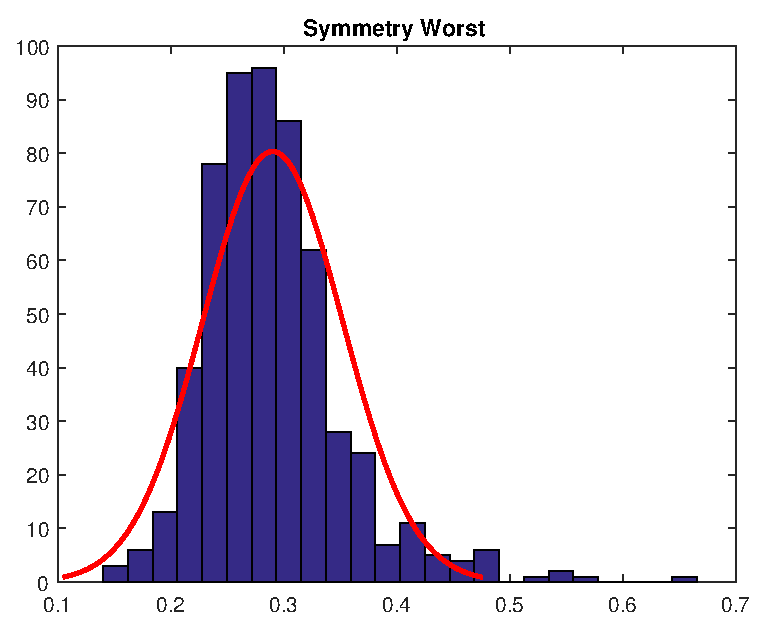
\includegraphics[width=\linewidth]{./img/symmetry_worst}
  \captionof{figure}{Worst}
  \label{fig:test2}
\end{minipage}
\end{figure}


\begin{table}[H]
\centering
\caption{Symmetry}
\label{my-label}
\begin{tabular}{lllll} \hline
              & symmetry\_mean & symmetry\_se & symmetry\_worst &  \\ \hline
Máximo        & 0.304          & 0.07895      & 0.6638          &  \\
Mínimo        & 0.106          & 0.007882     & 0.1565          &  \\
Média         & 0.181162       & 0.020542     & 0.290076        &  \\
Desvio padrão & 0.027414       & 0.008266     & 0.061867        &  \\
Percentil 25  & 0.1619         & 0.01516      & 0.2504          &  \\
Percentil 50  & 0.1792         & 0.01873      & 0.2822          &  \\
Percentil 75  & 0.1957         & 0.02348      & 0.3179          &  \\ \hline
\end{tabular}
\end{table}

Análise - A variável Symmetry mean possui um comportamento semelhante  a uma função Gaussiana e tanto Symmetry Standard Error, quanto Wosrt possuem valores máximos distantes da média.

\item Fractal Dimension
\begin{figure}[H]
\centering
  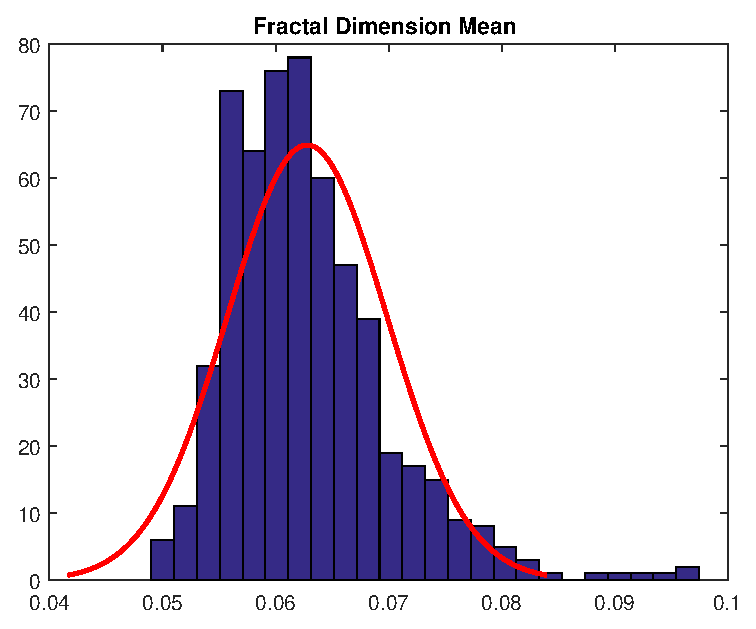
\includegraphics[width=.4\linewidth]{./img/fractal_dimension_mean}
  \captionof{figure}{Mean}
  \label{fig:test1}
\end{figure}%

\begin{figure}[H]
\centering
\begin{minipage}{.4\textwidth}
  \centering
  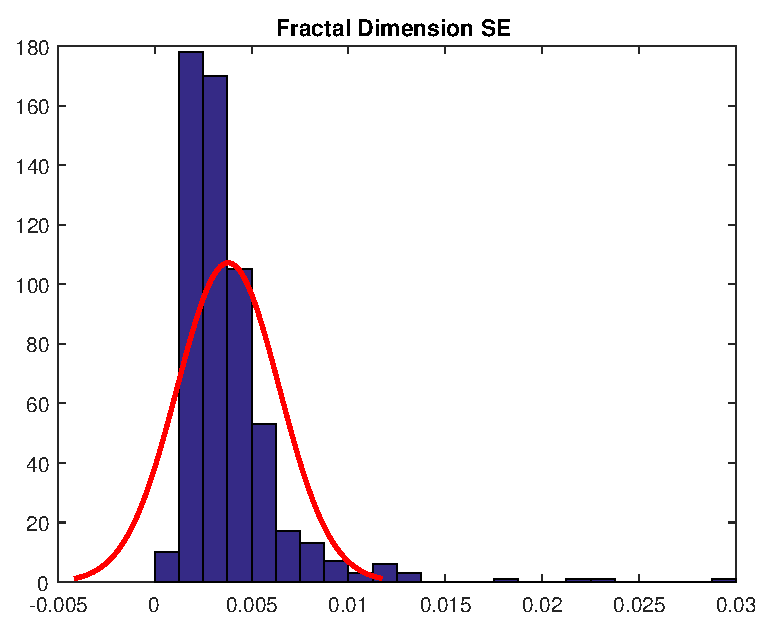
\includegraphics[width=\linewidth]{./img/fractal_dimension_se}
  \captionof{figure}{Standard Error}
  \label{fig:test1}
\end{minipage}%
\begin{minipage}{.4\textwidth}
  \centering
  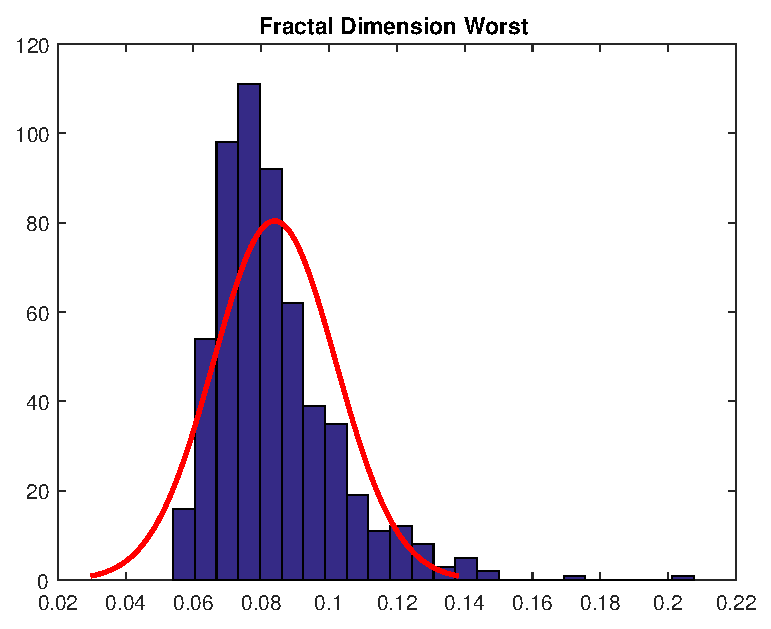
\includegraphics[width=\linewidth]{./img/fractal_dimension_worst}
  \captionof{figure}{Worst}
  \label{fig:test2}
\end{minipage}
\end{figure}
\end{itemize}

\begin{table}[H]
\centering
\caption{Fractal dimension}
\label{my-label}
\begin{tabular}{lllll} \hline
              & fractal\_dimension\_mean & fractal\_dimension\_se & fractal\_dimension\_worst &  \\ \hline
Máximo        & 0.09744                  & 0.02984                & 0.2075                    &  \\
Mínimo        & 0.04996                  & 0.000895               & 0.05504                   &  \\
Média         & 0.06279761               & 0.003795               & 0.083945817               &  \\
Desvio padrão & 0.007060363              & 0.002646               & 0.018061267               &  \\
Percentil 25  & 0.0577                   & 0.002248               & 0.07146                   &  \\
Percentil 50  & 0.06154                  & 0.003187               & 0.08004                   &  \\
Percentil 75  & 0.06612                  & 0.004558               & 0.09208                   &  \\ \hline
\end{tabular}
\end{table}

Análise:   Podemos ver que apartir da média, a ocorrência dos valores das váreiaveis vão  diminuindo conforme se distanciam da média.

A partir dos histogramas podemos avaliar que em geral não revelou características indesejáveis como distribuições multimodais. Conforme comentado algumas apresentaram assimetria.

\subsection{Matriz de Correlação}
\begin{figure}[H]
\centering
  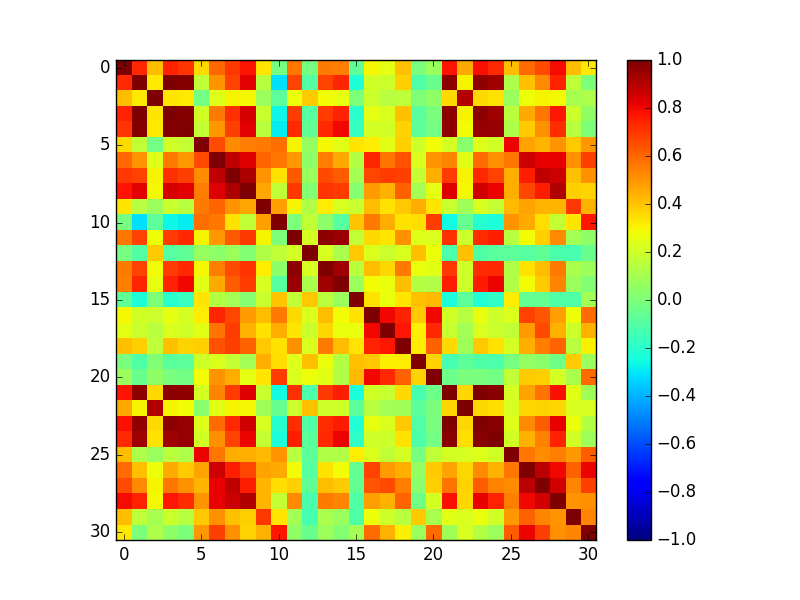
\includegraphics[width=\linewidth]{./img/corrcoef_range.png}
  \captionof{figure}{Matriz de Correlação}
  \label{fig:test1}
\end{figure}%

A partir da matriz podemos concluir que as seguintes variáveis estão fortemente correlacionadas (apresentam coeficiente de correlação acima de 0.9):
\begin{itemize}
	 \item Radius Mean, Perimeter Mean
	 \item Radius Mean, Area Mean
	 \item Radius Mean, Radius Worst
	 \item Radius Mean, Perimeter Worst
	 \item Radius Mean, Area Worst
	 \item Texture Mean, Texture Worst
	 \item Perimeter Mean, Area Mean
	 \item Perimeter Mean, Radius Worst
	 \item Perimeter Mean, Perimeter Worst
	 \item Perimeter Mean, Area Worst
	 \item Area Mean, Radius Worst
	 \item Area Mean, Perimeter Worst
	 \item Area Mean, Area Worst
	 \item Concavity Mean, Concave Points Mean
	 \item Concave Points Mean, Concave Points Worst
	 \item Radius SE, Perimeter SE
	 \item Radius SE, Area SE
	 \item Perimeter SE, Area SE
 	 \item Radius Worst, Perimeter Worst
	 \item Radius Worst, Area Worst
	 \item Perimeter Worst, Area Worst
    %\item Texture Mean, Area Mean
    %\item Texture Mean, Smoothness Mean
    %\item Texture Mean, Texture Worst
    %\item Texture Mean, Area Worst
    %\item Texture Mean, Smoothness Worst
    %\item Perimeter Mean, Perimeter Worst
    %\item Area Mean, Smoothness Mean
    %\item Area Mean, Texture Worst
    %\item Area Mean, Area Worst
    %\item Area Mean, Smoothness Worst
    %\item Smoothness Mean, Texture Worst
    %\item Smoothness Mean, Area Worst
    %\item Smoothness Mean, Smoothness Worst
    %\item Concave Points Mean, Symmetry Mean
    %\item Symmetry Mean, Symmetry Worst
    %\item Texture SE, Area SE
    %\item Texture SE, Smoothness SE
    %\item Area SE, Smoothness SE
    %\item Texture Worst, Area Worst
    %\item Texture Worst, Smoothness Worst
\end{itemize}

As seguintes variáveis apresentaram correlação negativa:

\begin{table}[H]
\centering
\begin{tabular}{c|c}
\hline
Variável A                & Variável B             \\
\hline
compactness\_mean         & perimeter\_mean        \\
radius\_se                & radius\_mean           \\
radius\_se                & texture\_mean          \\
radius\_se                & perimeter\_mean        \\
radius\_se                & area\_mean             \\
radius\_se                & smoothness\_mean       \\
perimeter\_se             & radius\_mean           \\
perimeter\_se             & texture\_mean          \\
perimeter\_se             & area\_mean             \\
perimeter\_se             & smoothness\_mean       \\
compactness\_se           & radius\_mean           \\
compactness\_se           & texture\_mean          \\
compactness\_se           & perimeter\_mean        \\
compactness\_se           & area\_mean             \\
compactness\_se           & smoothness\_mean       \\
fractal\_dimension\_se    & radius\_mean           \\
fractal\_dimension\_se    & texture\_mean          \\
fractal\_dimension\_se    & perimeter\_mean        \\
fractal\_dimension\_se    & area\_mean             \\
fractal\_dimension\_se    & smoothness\_mean       \\
radius\_worst             & radius\_mean           \\
radius\_worst             & texture\_mean          \\
radius\_worst             & perimeter\_mean        \\
radius\_worst             & area\_mean             \\
radius\_worst             & smoothness\_mean       \\
texture\_worst            & radius\_se             \\
texture\_worst            & perimeter\_se          \\
texture\_worst            & compactness\_se        \\
texture\_worst            & fractal\_dimension\_se \\
perimeter\_worst          & radius\_se             \\
perimeter\_worst          & compactness\_se        \\
perimeter\_worst          & fractal\_dimension\_se \\
area\_worst               & radius\_se             \\
area\_worst               & compactness\_se        \\
area\_worst               & perimeter\_se          \\
area\_worst               & fractal\_dimension\_se \\
smoothness\_worst         & radius\_se             \\
smoothness\_worst         & compactness\_se        \\
smoothness\_worst         & perimeter\_se          \\
smoothness\_worst         & fractal\_dimension\_se \\
compactness\_worst        & fractal\_dimension\_se \\
compactness\_worst        & perimeter\_se          \\
concavity\_worst          & perimeter\_se          \\
concavity\_worst          & compactness\_se        \\
concave points\_worst     & perimeter\_se          \\
concave points\_worst     & compactness\_se        \\
symmetry\_worst           & perimeter\_se          \\
symmetry\_worst           & compactness\_se        \\
symmetry\_worst           & fractal\_dimension\_se \\
fractal\_dimension\_worst & perimeter\_se          \\
fractal\_dimension\_worst & compactness\_se       
\end{tabular}
\end{table}
\subsection{Matriz de Distâncias} 

As figuras \ref{fig:distorig} e \ref{fig:zscore} mostram a matriz de distâncias, utilizando a Distância Euclidiana:
\[dist_E(\nu,\upsilon) = ||\nu-\upsilon||\]


\begin{figure}[H]
\centering
\begin{subfigure}{.5\textwidth}
  \centering
  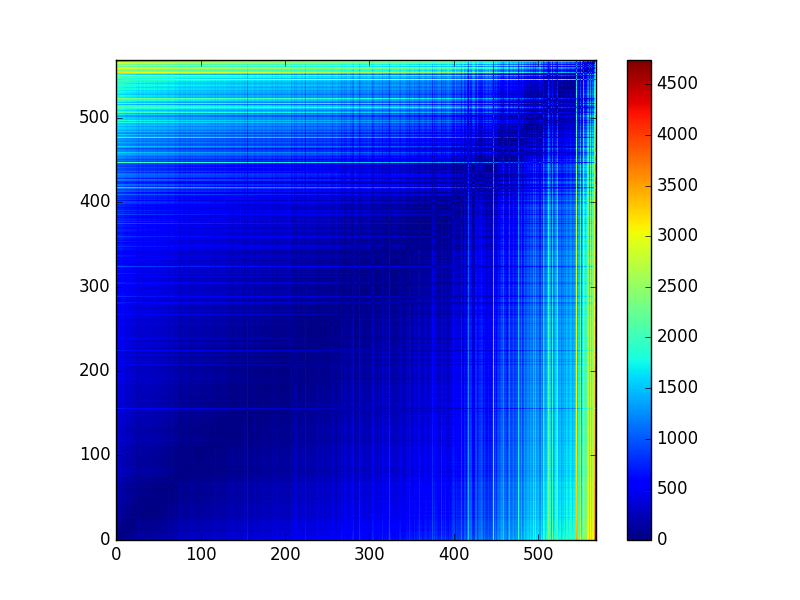
\includegraphics[width=\linewidth]{./img/distance_out}
  \caption{Antes da retirada de outliers}
  \label{fig:antes_out}
\end{subfigure}%
\begin{subfigure}{.5\textwidth}
  \centering
  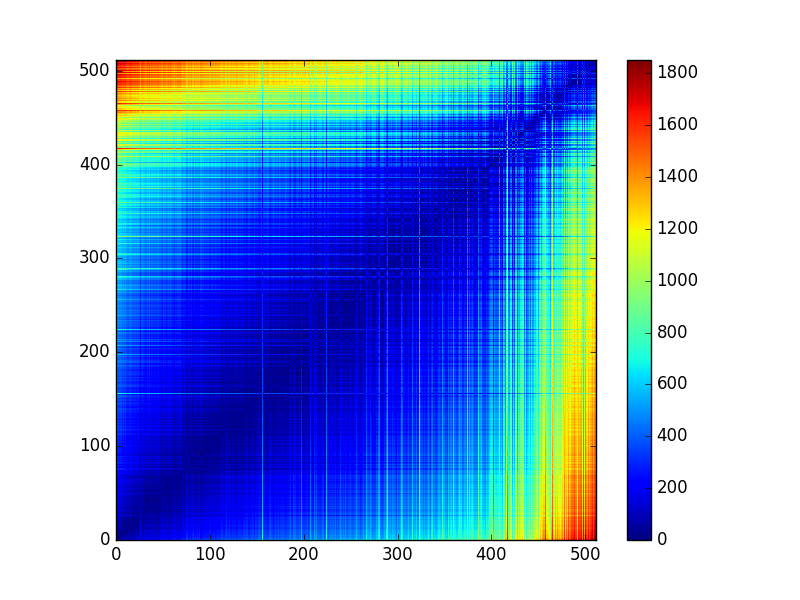
\includegraphics[width=\linewidth]{./img/distance_clean}
  \caption{Após da retirada de outliers}
  \label{fig:apos_out}
\end{subfigure}
\caption{Matriz de distâncias}
\label{fig:distorig}
\end{figure}

A matriz de distâncias para o conjunto de registros original pode ser observada na figura \ref{fig:antes_out}. Foi realizado o processo de retirada de outliers baseado na distância média $m_i = \frac{1}{N} \Sigma^N_{j=1} d_{ij}$. Foram removidos os $P_{out} = 10\%$ registros correspondentes aos maiores valores. A matriz de distâncias do conjunto de dados resultante pode ser vista na figura \ref{fig:apos_out}.

\begin{figure}[H]
\centering
\begin{subfigure}{.5\textwidth}
  \centering
  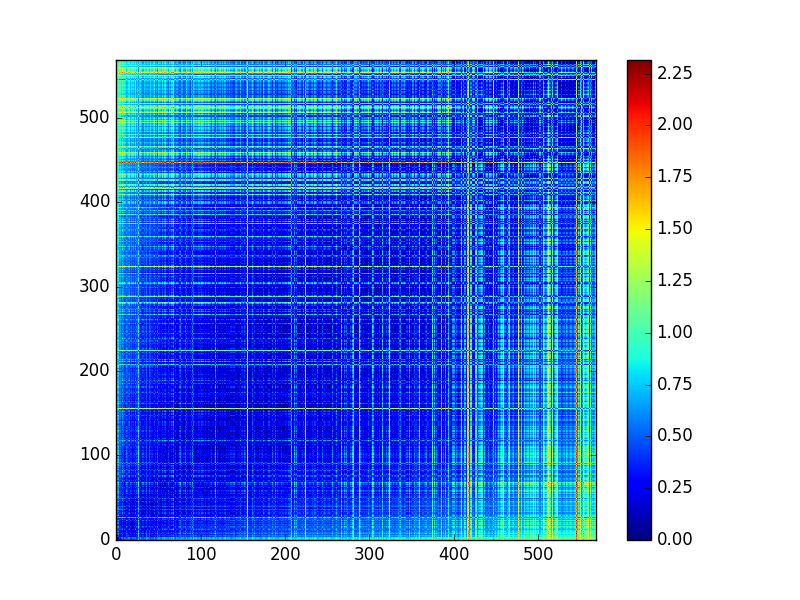
\includegraphics[width=\linewidth]{./img/dist_zscore_out}
  \caption{Antes da retirada de outliers}
  \label{fig:zantes_out}
\end{subfigure}%
\begin{subfigure}{.5\textwidth}
  \centering
  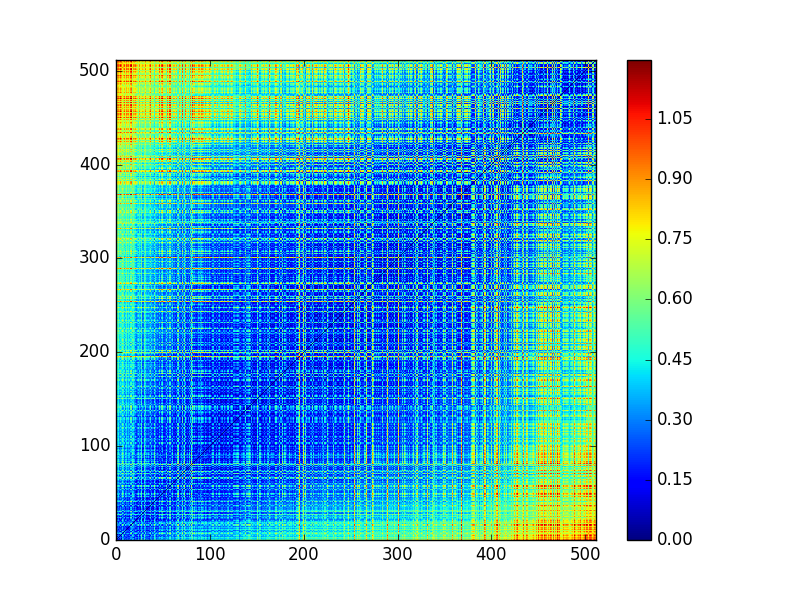
\includegraphics[width=\linewidth]{./img/distance_zscore_clean}
  \caption{Após da retirada de outliers}
  \label{fig:zapos_out}
\end{subfigure}
\caption{Matriz de distâncias com z-score}
\label{fig:zscore}
\end{figure}

Como o conjunto de dados contém variáveis em unidades e escalas diferentes, o que dificulta a avaliação da matriz de distâncias pois os outliers de algumas variáveis acabam dominando. Assim, foi feita uma padronização das variáveis por meio da estimativa z-score e a matriz de distâncias resultante pode ser vista na figura \ref{fig:zscore}.

\section{Formulação do Problema}
Consiste em um problema de classificação. Deseja-se desenvolver um classificador capaz de predizer a classe do registro (maligno ou benigno).

Para solução deste problema serão aplicados os modelos de classificação a seguir e avaliados os resultados.

\begin{itemize}
\item Classificador Bayesiano Simples
\item Classificador Bayesiano Quadrático
\item Regressão Logística
\item Perceptron Múltiplas Camadas
\end{itemize}

Para os testes a seguinte metodologia será usada. O dataset é dividido em uma razão de $67\%$ dos dados para treinamento e $33\%$ dos dados para teste. Para avaliar o desempenho do classificador, os resultados preditos pelo teste é comparado com os resultados reais e contabilizada a matriz de confusão. A partir dela são calculados as seguintes métricas:
\begin{itemize}
\item Acurácia
\item Erro global
\item Precisão 
\item Recuperação
\end{itemize}

\section{Apresentação da Tecnologia}
Para a implementação e execução dos algoritmos serão usadas as seguintes ferramentas, conforme se mostrarem mais adequadas para a tarefa em questão.

\subsection{Python}
A linguagem Python apresenta diversas bibliotecas úteis como:
\begin{itemize}
\item \textit{SciPy}: Ecossistema de softwares para matemática, ciência e engenharia. Contém os pacotes:
\begin{itemize}
\item \textit{NumPy}
\item \textit{matplotlib}
\item \textit{pandas}: Python Data Analysis Library
\end{itemize}
\item \textit{scikit-learn}: Machine Learning in Python
\end{itemize}

\subsection{Matlab}
Possui o seguinte \textit{Toolbox}
\begin{itemize}
\item Statistics and Machine Learning Toolbox
\end{itemize}

\section{Classificador Bayesiano Simples}

O Classificador Bayesiano baseia-se na aplicação do Teorema de Bayes com a suposição de independência entre cada par de variáveis. 

\section{Classificador Bayesiano Quadrático}
\section{Regressão Logística}
\section{Perceptron}
O Perceptron utiliza o modelo McCulloch-Pitts para o neurônio artificial. O processamento de cada unidade é dado por:
\[ u(t) = h(z(t)) = h \left( \theta_0 + \sum_{i=1}^n x_i(t) \theta_i \right) \]
onde:

$u(t)$: valor de ativação

$z(t)$: potencial de ativaçãos

$h$: função de ativação

$x_i(t)$: entradas do neurônio

O Perceptron incorpora o conceito de aprendizado, ou seja, se o padrão é classificado corretamente nenhum ajuste é realizado.
\section{Perceptron de Múltiplas Camadas (MLP)}
Uma rede-neural MLP apresenta uma camada de entrada que não realiza processamento, uma ou mais camadas intermediárias que realizam processamento e uma camada de saída que, num problema de classificação é o vetor com as estimativas das variáveis indicadoras. O modelo McCulloch-Pitts é utilizado nas unidades das camadas intermediárias e de saída.




\begin{table}[]
\centering
\caption{My caption}
\label{my-label}
\begin{tabular}{lllllll}
Máximo  & Mínimo   & Média    & Desvio Padrão & P 25 & P 50 & P 75 \\
28.11   & 6.981    & 14.13    & 3.524         & 11.7         & 13.37        & 15.78        \\
2.873   & 0.1115   & 0.4052   & 0.2773        & 0.2324       & 0.3242       & 0.4789       \\
36.04   & 7.93     & 16.27    & 4.833         & 13.01        & 14.97        & 18.79        \\
39.28   & 9.71     & 19.29    & 4.301         & 16.17        & 18.84        & 21.8         \\
4.885   & 0.3602   & 1.217    & 0.5516        & 0.8339       & 1.108        & 1.474        \\
49.54   & 12.02    & 25.68    & 6.146         & 21.08        & 25.41        & 29.72        \\
188.5   & 43.79    & 91.97    & 24.3          & 75.17        & 86.24        & 104.1        \\
21.98   & 0.757    & 2.866    & 2.022         & 1.606        & 2.287        & 3.357        \\
251.2   & 50.41    & 107.3    & 33.6          & 84.11        & 97.66        & 125.4        \\
2501    & 143.5    & 654.9    & 351.9         & 420.3        & 551.1        & 782.7        \\
542.2   & 6.802    & 40.34    & 45.49         & 17.85        & 24.53        & 45.19        \\
4254    & 185.2    & 880.6    & 569.4         & 515.3        & 686.5        & 1084         \\
0.1634  & 0.05263  & 0.09636  & 0.01406       & 0.08637      & 0.09587      & 0.1053       \\
0.03113 & 0.001713 & 0.007041 & 0.003003      & 0.005169     & 0.00638      & 0.008146     \\
0.2226  & 0.07117  & 0.1324   & 0.02283       & 0.1166       & 0.1313       & 0.146        \\
0.3454  & 0.01938  & 0.1043   & 0.05281       & 0.06492      & 0.09263      & 0.1304       \\
0.1354  & 0.002252 & 0.02548  & 0.01791       & 0.01308      & 0.02045      & 0.03245      \\
1.058   & 0.02729  & 0.2543   & 0.1573        & 0.1472       & 0.2119       & 0.3391       \\
0.4268  & 0		   & 0.0888   & 0.07972       & 0.02956      & 0.06154      & 0.1307         \\
0.396   & 0  	   & 0.03189  & 0.03019       & 0.01509      & 0.02589      & 0.04205      \\
1.252   & 0        & 0.2722   & 0.2086        & 0.1145       & 0.2267       & 0.3829       \\
0.2012  & 0        & 0.04892  & 0.0388        & 0.02031      & 0.0335       & 0.074        \\
0.05279 & 0  	   & 0.0118   & 0.00617       & 0.007638     & 0.01093      & 0.01471      \\
0.291   & 0		   & 0.1146   & 0.06573       & 0.06493      & 0.09993      & 0.1614       \\
0.304   & 0.106    & 0.1812   & 0.02741       & 0.1619       & 0.1792       & 0.1957       \\
0.07895 & 0.007882 & 0.02054  & 0.008266      & 0.01516      & 0.01873      & 0.02348      \\
0.6638  & 0.1565   & 0.2901   & 0.06187       & 0.2504       & 0.2822       & 0.3179       \\
0.09744 & 0.04996  & 0.0628   & 0.00706       & 0.0577       & 0.06154      & 0.06612      \\
0.02984 & 0.000895 & 0.003795 & 0.002646      & 0.002248     & 0.003187     & 0.004558     \\
0.2075  & 0.05504  & 0.08395  & 0.01806       & 0.07146      & 0.08004      & 0.09208     
\end{tabular}
\end{table}


\end{document}
